\section{BGP routing table}
\label{sec:bgp}

In this section we present extensive evaluation of the global routing table
from 2003 to 2009. The first point of our interest is to analyze contribution
of causes to the global routing table growth. That is, we determine how well
ISPs tend to use an allocated address space and how this address space is
subdivided. The second point of interest is to analyze the contents of the BGP
routing table itself. This include an analysis of a level of the overlapping
IP prefix announcements (i.e., how many individual prefixes are also parts of
the bigger prefixes, present in the same routing table). We also show the
stability of the routing table contents. For this purpose, we calculate time
periods during which each individual prefix was visible by the selected BGP
monitor. Finally, we present an evaluation of the BGP routing table entries in
geographical layer, including a tabular and graphical representation of the
BGP entries and numbers of IP addresses, covered by these BGP entries, each
country contributes to the global routing table.

%%%%%%%%%%%%%%%%%%%%%%%%%%%%%%%%%%%%%%%%%%%%%%%%%%%%%%%%%%%%%%%%%%%%%%%%%%%%%
%%%%%%%%%%%%%%%%%%%%%%%%%%%%%%%%%%%%%%%%%%%%%%%%%%%%%%%%%%%%%%%%%%%%%%%%%%%%%
%%%%%%%%%%%%%%%%%%%%%%%%%%%%%%%%%%%%%%%%%%%%%%%%%%%%%%%%%%%%%%%%%%%%%%%%%%%%%
\subsection{Analysis of BGP table growth factors}
%%%%%%%%%%%%%%%%%%%%%%%%%%%%%%%%%%%%%%%%%%%%%%%%%%%%%%%%%%%%%%%%%%%%%%%%%%%%%
%%%%%%%%%%%%%%%%%%%%%%%%%%%%%%%%%%%%%%%%%%%%%%%%%%%%%%%%%%%%%%%%%%%%%%%%%%%%%
%%%%%%%%%%%%%%%%%%%%%%%%%%%%%%%%%%%%%%%%%%%%%%%%%%%%%%%%%%%%%%%%%%%%%%%%%%%%%

The BGP routing table growth is much faster than growth of the number of the
allocated IP blocks (see Figure~\ref{fig:BGP vs RIR}). Currently, the average
number of entries in the global routing table in more than 3 times more than
total number of allocated IP blocks. This increase has dual nature. Firstly,
ISPs tend to subdivide allocated IP blocks into several individual prefixes
and announce them separately. For example, such behavior is very typical for
the transnational providers and providers which lend parts of allocated
address space to its customers, which, in their case, independently announce
lent IP address block. Secondly, various traffic engineering techniques
(traffic balancing, multihoming, etc) create situations when the same address
block is covered by several announced prefixes.

\subsubsection{IP block fragmentation}

Figure~\ref{fig:fragmentation} presents a correlation between allocated IP
blocks and announced IP prefixes. The \emph{matched} curve on the figure
represents IP blocks, which are announced in the exact form as they were
issued by the RIRs. An example of the matched prefix announcement is when an
ISP allocates a block of 1,024 IP addresses (equivalent to /22 block) and then
globally announces this block as a single /22 prefix. As one can see,
currently the number of matched prefixes accounts only 1/6$^{th}$ of the total
number of BGP entries, and this ratio tends to be even smaller in future.

\begin{figure}[htbp]
	\centering
		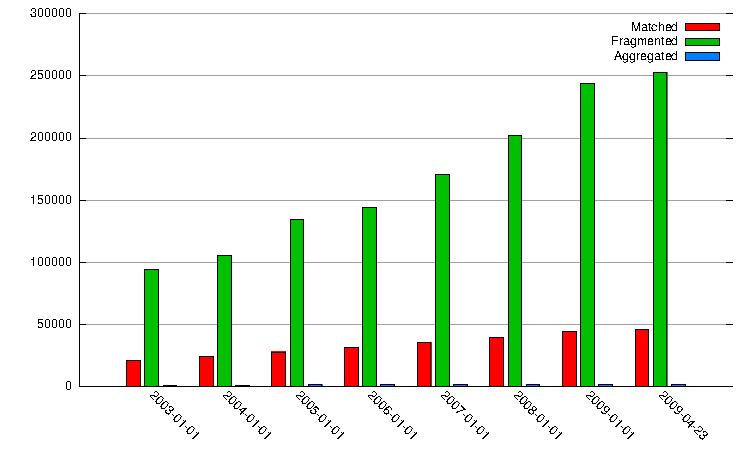
\includegraphics[width=\columnwidth]{05_matched_fragmented/frag-3}
	\caption{Dynamics of matched, fragmented, and aggregated IP prefixes in BGP announcements}
	\label{fig:fragmentation}
\end{figure}

This consideration allows us to make a conclusion that ISPs are not willing to
use allocated address space as is. Instead, they for some reason (e.g.,
geographical dispersion) split up allocated block into a number of sub-blocks
and announce each of the independently. The \emph{fragmented} curve in
Figure~\ref{fig:fragmentation} represents these split up blocks, which
accounts more than 83\% of all entries in global routing table. That is, the
allocated IP block fragmentation is a primary concern for the future BGP
protocol scalability.

The last curve, \emph{aggregated}, represents IP prefix announcements, which
cover several allocated IP blocks. That is, in contrast to the fragmentation,
ISPs, which has several adjacent IP block allocations, are willing to announce
them as a single IP prefix. Unfortunately, the aggregation technique aimed to
reduce hiking number of entries in routing table does not work. In 2003 a
number of aggregated prefixes was 1,400 and this number increased marginally
to nearly 2,000 prefixes in 2009, which is nothing comparing to the total
number of prefixes in the BGP routing table ($\approx$300k).

One surprising conclusion can be made from this analysis. ISPs do not tend to
globally announce the allocated IP space in the original form, no matter of
what size IP block is allocated. This conclusion can serve as a base of
different conclusion concerning future IPv6 deployment. Without a major change
in the BGP protocol, an increase of the allocation IP block size (according to
the current RIRs policy, the minimum allocation IPv6 block is
/32\cite{APNIC:2009:IPv6-Address}) will not help to significantly
reduce the size of global routing table. The only targets for the reduction
are matched IP prefixes (i.e., ISPs which currently use all allocated IP space
as a single block will likely to use a bigger IPv6 space also as a single
block). That is, the upper bound of IP space level optimization is limited by
the number of matched prefixes (less than 17\% of all prefixes).

\subsubsection{Duplicate announcements of IP blocks}

BGP routing table has a consistent trends of containing a large portion of
prefixes, which duplicate each other (Figure~\ref{fig:covered}). In theory,
the IP address coverage duplication in a routing table, where the actual route
is calculated by matching the destination address with the longest available
prefix, is one of the effective ways to reduce a size of the routing table
itself. For example, consider an ISP owning a /8 address block and wanting to
route some /24 block using a different path than the rest of the block. It is
much effective to use a small duplication of address space and only two
entries in routing table, instead of no duplication and 65,536 individual
entries.

\begin{figure}[htbp]
	\centering
		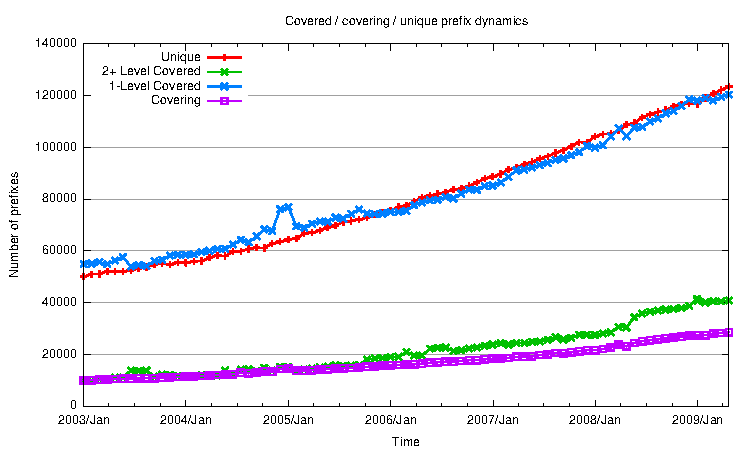
\includegraphics[width=\columnwidth]{06_covered/cover-3}
	\caption{Dynamics of covered, covering, and unique IP prefixes in BGP announcements}
	\label{fig:covered}
\end{figure}

The reality shows that the fundamental IP routing feature of longest prefix
matching is used very extensively. As we can see in Figure~\ref{fig:covered}
(\emph{1 level} curves) number of IP prefixes in BGP table which are covered
by exactly one bigger prefix is nearly the same as number of unique prefixes
(i.e., base prefixes). Moreover, there are substantial amount of prefixes
which has several layers of coverage (several duplication levels, \emph{2+
level} curve).

This high numbers indicate a presence of some additional (besides the
theoretical routing table optimization) incentives for prefix duplication. One
of such factors is a multi-provider connection for end-networks (so called,
multihoming of \emph{stub networks}). According to Oliveira et al.
\cite{Oliveira:2007:Observing-the-evolution}, more than 70\% of all
announcements belongs to multihomed stub networks. In other words, the global
routing table was adopted to serve local or semi-local routing interests of
the majority of customers. It is very unlikely that a customer (a stub
network) connects to providers which are very spaced from each other in the
terms of routing. The conclusion is that if we want to significantly reduce a
size of the BGP routing table, we should find ways to eliminate IP prefix
fragmentation incentives. For example, by providing separate means for
multihoming and traffic engineering tasks.

%%%%%%%%%%%%%%%%%%%%%%%%%%%%%%%%%%%%%%%%%%%%%%%%%%%%%%%%%%%%%%%%%%%%%%%%%%%%%
%%%%%%%%%%%%%%%%%%%%%%%%%%%%%%%%%%%%%%%%%%%%%%%%%%%%%%%%%%%%%%%%%%%%%%%%%%%%%
%%%%%%%%%%%%%%%%%%%%%%%%%%%%%%%%%%%%%%%%%%%%%%%%%%%%%%%%%%%%%%%%%%%%%%%%%%%%%
\subsection{Analysis of the BGP table contents}
%%%%%%%%%%%%%%%%%%%%%%%%%%%%%%%%%%%%%%%%%%%%%%%%%%%%%%%%%%%%%%%%%%%%%%%%%%%%%
%%%%%%%%%%%%%%%%%%%%%%%%%%%%%%%%%%%%%%%%%%%%%%%%%%%%%%%%%%%%%%%%%%%%%%%%%%%%%
%%%%%%%%%%%%%%%%%%%%%%%%%%%%%%%%%%%%%%%%%%%%%%%%%%%%%%%%%%%%%%%%%%%%%%%%%%%%%

Analysis of the BGP routing table contents reveals the current trends and
demands for the IP space. Later in this section we will show an analysis of a
announced prefix size distribution, IP prefix longevity in global BGP
announcements, and geographical distribution of the IP space.

\subsubsection{Lengths of announced IP prefixes}

One of the most critical questions in global routing system is what is the
optimal length of IP prefix to allocate to customers, and what is the optimal
algorithm to select a right prefix to allocate (e.g., how many space should be
reserved after allocated block for the case of the repeated requests from the
same customer). There is a number of solutions to resolve the latter question,
including sequential and bisection allocation schemes, and GAP algorithm
\cite{Wang:2007:Reduce-IP-Address}. The former question is still open.

Figure~\ref{fig:bgp prefix distribution} presents a distribution of the
announced prefix length. The majority of the global routing table entries are
/24-length prefixes (more than 53\% of entries). And during the last 6 years a
number of /24 prefixes practically doubled. At the same time, number of
actually allocated /24 blocks is 4 times smaller (see Figure~\ref{fig:IP
allocations}). This one more time highlights the fact, that a very big number
of stub networks (i.e., relatively small customer networks) are using
announcements of small address blocks to implement multi-provider
connectivity.

\begin{figure}[htbp]
	\centering
		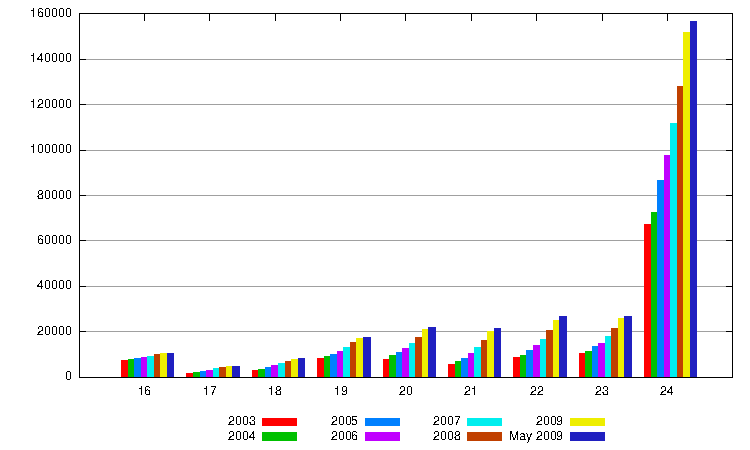
\includegraphics[width=\columnwidth]{02_prefixes/01_bgp_prefixes_zoom}
	\caption{Distribution of announced IP prefix lengths}
	\label{fig:bgp prefix distribution}
\end{figure}

Prefix length of /16 -- /23 has relatively the same level of popularity in the
global routing table, where /17 and /18 has a least popularity. The most
dynamic prefixes from this group are /20 and /21 (growth 2.8 and 3.7 times
respectively), and the least dynamic -- /16 (growth 1.4 times). Another very
interesting observation is for /16 prefix. From the most influential prefixes
(in terms of number of consuming entries in global routing table), the /16
prefix is the only one having a number of global announcements practically
equal to a number of allocations.

The rest of the prefixes has a marginal presence in the global routing table
(total less than 8000 prefixes). This fact shows a small number of entities
having a small (prefixes $<$/16) prefixes and a small number of a tiny
(prefixes $>$/24) customer networks with a multi-provider connectivity.

The results of in this section are additional evidence of the tight
relationship between global routing table growth and IP space fragmentation
and duplication. If we can suppress majority of non-global related
announcements (i.e., bursts of /24 prefixes due to local traffic engineering,
local and semi-local multihoming support, etc), the size of the global routing
table would be significantly reduced.

\subsubsection{Longevity distribution of BGP entries}

Another aspect of the BGP announcement analysis is determining the stability
of the global routing table. In Figure~\ref{fig:bgp ages} presented
distribution of the prefix longevity. The main observation from the graph is
that more than 15\% of the global routing table never changes. On the other
hand, about 15\% (if we compare to the global routing table size in 2009) of
the prefixes were active only for short period of time. A part of these
short-lived prefixes, probably, belongs to spammers who hijack somebody else's
(or nobody's) prefix and announce it for the time to send virtually
untraceable spam messages
\cite{Ramachandran:2006:Understanding-the-network-level}. Some part of the
short-lived prefixes could be explained by the configuration errors. The rest
is, probably, explained by the normal BGP operation where some prefix become
visible only in the case of the primary channel error.

\begin{figure}[htbp]
	\centering
		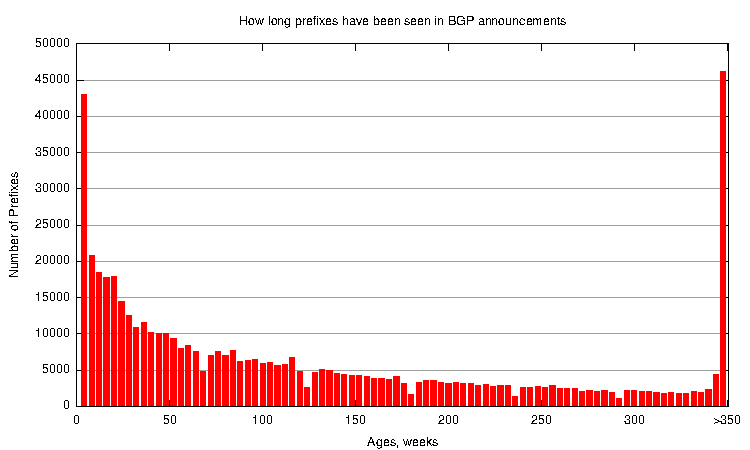
\includegraphics[width=\columnwidth]{08_ages/ages-4}
	\caption{Longevity of prefixes in BGP announcements}
	\label{fig:bgp ages}
\end{figure}

As one can notice from Figure~\ref{fig:bgp ages}, prefix longevity
distribution to some extent is following the exponential distribution
function. That is, besides the fixed number of highly stable routes (15\%), it
is unlikely that some route is visible too long. And in opposite direction,
announced prefixes are likely to have small longevity. This observation shows
the substantial level of the global routing table dynamics.

\subsubsection{BGP announcements by geographical region}
% One other direction of our BGP routing system study deals with
% characteristics of the allocations and announcements themselves. These are
% in the areas of geography and age. Some of the new areas we will examine to
% monitor where allocation activity is happening, and for how long a time on
% average. Thus, seventh, we will give a year-on-year comparison of prefix
% allocations and prefix announcements by major countries, including Russia,
% Japan, major countries of Asia, and broad regions such as the European
% Union, North America, and Africa.
% The last, but not least topic 

As a final analysis of the global routing table content, we present a country-based analysis for the number of globally announced IP prefixes. The analysis of a fixed time snapshots points out the major contributers to the global routing table and gives an understanding of the Internet penetration throughout the world. 

Table~\ref{tab:top25 bgp prefixes 2003} presents a top 25 contributors to the
global routing table in 2003 with the indications of what actual IP address
space is covered by the sets of announced prefixes. Table~\ref{tab:top25 bgp
ip space 2003} gives an alternative representation for the BGP data snapshot
from 2003, where countries are ordered by the number of used (announced) IP
space. Due to the limited nature of our IP prefix country association
technique (see Section~\ref{sec:data sets}), there is a considerable portion
of prefixes for which we could not establish such association. In fact, in
2003 the globally announced prefixes with undetermined ownership were the
second most contributors to the routing table after United States. Third and
forth place for the contribution to the routing table in 2003 were taken by
Australia and Canada. It should be mentioned, that geographical distribution
of announced IP prefixes and announced IP space has stable quasi-exponential
distribution (Figure~\ref{fig:prefix distr} and Figure~\ref{fig:size distr})

\begin{figure}[htbp]
	\centering
		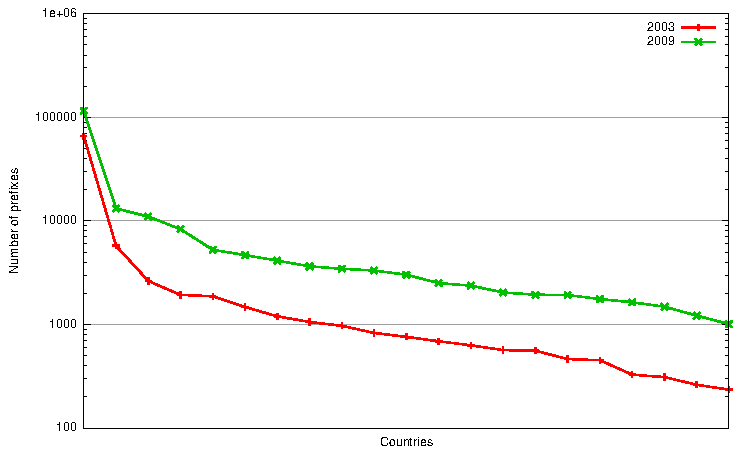
\includegraphics[width=\columnwidth]{01_bgp_ip_size/prefix-distr}
	\caption{Geographical distribution of globally announced IP prefixes (log scale)}
	\label{fig:prefix distr}
\end{figure}

\begin{figure}[htbp]
	\centering
		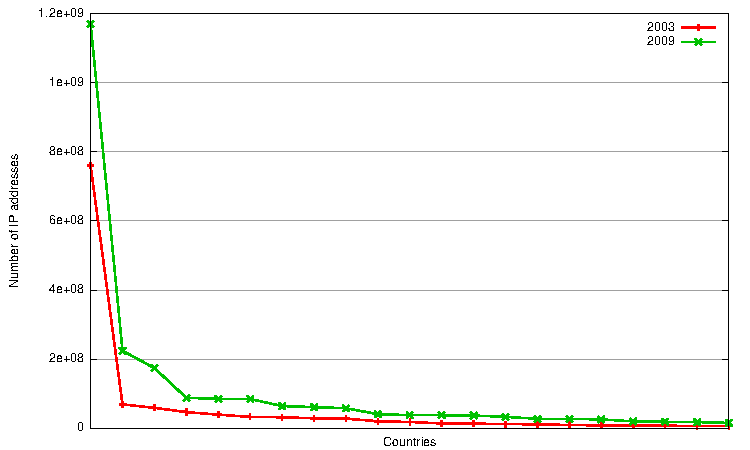
\includegraphics[width=\columnwidth]{01_bgp_ip_size/size-distr}
	\caption{Geographical distribution of globally announced IP space (log scale)}
	\label{fig:size distr}
\end{figure}

Table~\ref{tab:top25 bgp prefixes 2009} and Table~\ref{tab:top25 bgp ip space
2009} present an up-to-date estimate of top 25 contributors to the global
routing table and top 25 countries with the most announced address space. As
we can see, a number of prefixes with undetermined ownership (and a
corresponding IP space) decreased twice. At the same time all countries show a
substantial growth BGP table usage. However, United States saved its leader
positions, the rest of the table has significant changes. South Korea, China,
Australia, and India became the second major contributors to the size of
global routing table. At the same time, China, Japan, European Union, Germany,
and South Korea are countries with the most announced address space. This
observation highlight the fact that some countries are tend to extensively use
an allocated address space (e.g., in South Korea one prefix covers on average
5,900 addresses), and some are extremely efficient from BGP point of view
(e.g., in Japan one prefix covers on average 37,200 addresses). If this
difference in usage efficiency occur because of additional government
regulations, than for future IPv6 deployment, we should consider an
establishment of similar global regulations.

As an alternative way to represent each country contribution to the global
routing table, we present color-coded diagrams in Figures~\ref{fig:bgp
prefixes 2003}--\ref{fig:bgp ip space asia 2009}. The figure pairs
(Figure~\ref{fig:bgp prefixes 2003} and Figure~\ref{fig:bgp prefixes 2009},
Figure~\ref{fig:bgp ip space 2003} and Figure~\ref{fig:bgp ip space 2009})
allows trace the regional Internet growth dynamics. Figure~\ref{fig:bgp
prefixes asia 2009} and Figure~\ref{fig:bgp ip space asia 2009} one more time
emphasize different effectiveness of IP space utilization (e.g., Japan
comparing to India of South Korea has much more addresses per announced
prefix).


\begin{table*}[p]
%%%%%%%%%%%%%%%%%%%%%%%%%%%%%%%%%%%%%%%%%%%%%%%%%%%%%%%%%%%%%%%%%%%%%%%%%%%%%%%%
%% TOP announced prefixes
%%%%%%%%%%%%%%%%%%%%%%%%%%%%%%%%%%%%%%%%%%%%%%%%%%%%%%%%%%%%%%%%%%%%%%%%%%%%%%%%
\begin{minipage}[t]{0.48\textwidth}
% \begin{table}[p]
	\begin{center}
	\caption{Top 25 countries with the most number of announced prefixes in BGP table on \textbf{January 1, 2003}}
	\label{tab:top25 bgp prefixes 2003}
	\begin{tabular}{|l||l|r|r|} %\hline
		\hline
		&      \bf Country		&    Prefixes   &       IP space 		\tabularnewline \hline 
1       &       US      		&       65849   &       759,792,816     \tabularnewline %\hline
2       &       \emph{Unknown}	&       6258    &       68,926,314      \tabularnewline %\hline
3       &       Australia       &       5762    &       17,822,159      \tabularnewline %\hline
4       &       Canada  		&       5612    &       38,912,924      \tabularnewline %\hline
5       &       Japan   		&       2633    &       58,905,280      \tabularnewline %\hline
6       &       South Korea     &       2441    &       27,334,687      \tabularnewline %\hline
7       &       Germany			&       1934    &       46,556,556      \tabularnewline %\hline
8       &       India  			&       1931    &       2,943,040       \tabularnewline %\hline
9       &       UK     			&       1873    &       32,626,649      \tabularnewline %\hline
10      &       China  			&       1615    &       28,522,130      \tabularnewline %\hline
11      &       Argentina       &       1477    &       2,017,448       \tabularnewline %\hline
12      &       Hong Kong       &       1261    &       5,621,473       \tabularnewline %\hline
13      &       Sweden  		&       1198    &       11,280,533      \tabularnewline %\hline
14      &       France  		&       1148    &       31,320,040      \tabularnewline %\hline
15      &       Mexico  		&       1059    &       5,275,520       \tabularnewline %\hline
16      &       Romania 		&       994     &       667,136 		\tabularnewline %\hline
17      &       Russia  		&       972     &       5,911,712       \tabularnewline %\hline
18      &       Chile   		&       834     &       2,098,161       \tabularnewline %\hline
19      &       Indonesia       &       830     &       1,170,560       \tabularnewline %\hline
20      &       Italy   		&       791     &       13,324,288      \tabularnewline %\hline
21      &       Brazil  		&       760     &       11,580,416      \tabularnewline %\hline
22      &       Taiwan  		&       708     &       13,448,168      \tabularnewline %\hline
23      &       Netherlands     &       689     &       19,939,341      \tabularnewline %\hline
24      &       European Union  &       687     &       2,707,383       \tabularnewline %\hline
25      &       Finland 		&       630     &       7,307,018       \tabularnewline %\hline
% 26      &       South Africa    &       618     &       5,762,180       \tabularnewline %\hline
% 27      &       New Zealand     &       566     &       3,828,620       \tabularnewline %\hline
% 28      &       Switzerland     &       560     &       7,937,424       \tabularnewline %\hline
% 29      &       Thailand        &       559     &       1,877,060       \tabularnewline %\hline
% 30      &       Spain   		&       511     &       8,921,568       \tabularnewline %\hline
	\hline
	\end{tabular}
	\end{center}
% \end{table}
\end{minipage}
%
\quad
%
\begin{minipage}[t]{0.48\textwidth}
% \begin{table}[p]
	\begin{center}
	\caption{Top 25 countries with the most number of announced prefixes in BGP table on \textbf{April 23, 2009}}
	\label{tab:top25 bgp prefixes 2009}
	\begin{tabular}{|l||l|r|r|r|}
		\hline
		&      \bf Country		& \bf Prefixes  &       \bf IP space 	& \bf Change$^{*}$ 	\tabularnewline \hline 
1       &       US      		&       115780  &       1,170,481,177   & 1.54			\tabularnewline %\hline
2       &       South Korea     &       14308   &       84,553,300      & 3.09			\tabularnewline %\hline
3       &       China  			&       13188   &       223,990,021     & 7.85			\tabularnewline %\hline
4       &       Australia       &       11329   &       37,818,072      & 2.12			\tabularnewline %\hline
5       &       India   		&       11022   &       17,575,040      & 5.97			\tabularnewline %\hline
6       &       Russia  		&       8650    &       26,664,224      & 4.51			\tabularnewline %\hline
7       &       Canada  		&       8328    &       57,471,348      & 1.48			\tabularnewline %\hline
8       &       Romania 		&       5729    &       7,348,881       & 11.02			\tabularnewline %\hline
9       &       UK      		&       5269    &       63,871,082      & 1.96			\tabularnewline %\hline
10      &       European Union  &       4937    &       87,825,582      & 32.44			\tabularnewline %\hline
11      &       Japan   		&       4674    &       173,789,965     & 2.95			\tabularnewline %\hline
12      &       Brazil  		&       4643    &       40,429,504      & 3.49			\tabularnewline %\hline
13      &       Argentina       &       4142    &       9,721,411       & 4.82			\tabularnewline %\hline
14      &       Germany 		&       4035    &       84,904,642      & 1.82			\tabularnewline %\hline
15      &       Mexico  		&       3648    &       19,583,832      & 3.71			\tabularnewline %\hline
16      &       Indonesia       &       3562    &       5,248,256       & 4.48			\tabularnewline %\hline
17      &       Hong Kong       &       3459    &       14,764,300      & 2.63			\tabularnewline %\hline
18      &       \emph{Unknown}	&       3393    &       37,265,411      & 				\tabularnewline %\hline
19      &       Bulgaria        &       3325    &       4,439,040       & 7.72			\tabularnewline %\hline
20      &       Colombia        &       3029    &       4,901,340       & 11.86			\tabularnewline %\hline
21      &       Ukraine 		&       3028    &       5,547,136       & 7.67			\tabularnewline %\hline
22      &       Egypt  			&       2992    &       3,854,848       & 4.60			\tabularnewline %\hline
23      &       France 			&       2511    &       61,070,996      & 1.95			\tabularnewline %\hline
24      &       Taiwan 			&       2511    &       36,623,744      & 2.72			\tabularnewline %\hline
25      &       Chile  			&       2375    &       6,101,376       & 2.91			\tabularnewline %\hline
% 26      &       Poland 			&       2341    &       15,122,881      & 4.06			\tabularnewline %\hline
% 27      &       Thailand        &       2039    &       7,210,800       & 3.84			\tabularnewline %\hline
% 28      &       Spain   		&       1989    &       25,315,136      & 2.84			\tabularnewline %\hline
% 29      &       Sweden  		&       1942    &       18,532,345      & 1.64			\tabularnewline %\hline
% 30      &       Turkey  		&       1940    &       14,309,632      & 6.41			\tabularnewline %\hline
	\hline
	\end{tabular}
	\end{center}
	
	\small	$^{*}$ -- Relative change in number of prefixes in BGP announcements from January 1, 2003 and April 23, 2009
% \end{table}
\end{minipage}

\vspace{1cm}

%%%%%%%%%%%%%%%%%%%%%%%%%%%%%%%%%%%%%%%%%%%%%%%%%%%%%%%%%%%%%%%%%%%%%%%%%%%%%%%%
%% TOP announced IP space
%%%%%%%%%%%%%%%%%%%%%%%%%%%%%%%%%%%%%%%%%%%%%%%%%%%%%%%%%%%%%%%%%%%%%%%%%%%%%%%%
\begin{minipage}[t]{0.48\textwidth}
% \begin{table}[p]
	\begin{center}
	\caption{Top 25 countries with the most number of announced IP space in BGP table on \textbf{January 1, 2003}}
	\label{tab:top25 bgp ip space 2003}
	\begin{tabular}{|l||l|r|r|}
		\hline
		&      \bf Country		&    Prefixes   &       IP space 		\tabularnewline \hline 
1       &       US      		&       65849   &       759,792,816     \tabularnewline %\hline
2       &       \emph{Unknown} 	&       6258    &       68,926,314      \tabularnewline %\hline
3       &       Japan   		&       2633    &       58,905,280      \tabularnewline %\hline
4       &       Germany 		&       1934    &       46,556,556      \tabularnewline %\hline
5       &       Canada  		&       5612    &       38,912,924      \tabularnewline %\hline
6       &       UK      		&       1873    &       32,626,649      \tabularnewline %\hline
7       &       France  		&       1148    &       31,320,040      \tabularnewline %\hline
8       &       China   		&       1615    &       28,522,130      \tabularnewline %\hline
9       &       South Korea     &       2441    &       27,334,687      \tabularnewline %\hline
10      &       Netherlands     &       689     &       19,939,341      \tabularnewline %\hline
11      &       Australia       &       5762    &       17,822,159      \tabularnewline %\hline
12      &       Taiwan  		&       708     &       13,448,168      \tabularnewline %\hline
13      &       Italy   		&       791     &       13,324,288      \tabularnewline %\hline
14      &       Brazil  		&       760     &       11,580,416      \tabularnewline %\hline
15      &       Sweden  		&       1198    &       11,280,533      \tabularnewline %\hline
16      &       Spain   		&       511     &       8,921,568       \tabularnewline %\hline
17      &       Switzerland     &       560     &       7,937,424       \tabularnewline %\hline
18      &       Norway  		&       262     &       7,591,936       \tabularnewline %\hline
19      &       Finland 		&       630     &       7,307,018       \tabularnewline %\hline
20      &       Russia  		&       972     &       5,911,712       \tabularnewline %\hline
21      &       South Africa    &       618     &       5,762,180       \tabularnewline %\hline
22      &       Hong Kong       &       1261    &       5,621,473       \tabularnewline %\hline
23      &       Austria 		&       317     &       5,405,664       \tabularnewline %\hline
24      &       Mexico  		&       1059    &       5,275,520       \tabularnewline %\hline
25      &       Denmark 		&       196     &       4,169,984       \tabularnewline %\hline
% 26      &       New Zealand     &       566     &       3,828,620       \tabularnewline %\hline
% 27      &       Belgium 		&       175     &       3,796,224       \tabularnewline %\hline
% 28      &       Poland  		&       273     &       3,721,216       \tabularnewline %\hline
% 29      &       Malaysia        &       235     &       3,182,400       \tabularnewline %\hline
% 30      &       India   		&       1931    &       2,943,040       \tabularnewline %\hline
	\hline
	\end{tabular}
	\end{center}
	\ \newline\ \newline
% \end{table}
\end{minipage}
%
\quad
%
\begin{minipage}[t]{0.48\textwidth}
% \begin{table}[p]
	\begin{center}
	\caption{Top 25 countries with the most number of announced IP space in BGP table on \textbf{April 23, 2009}}
	\label{tab:top25 bgp ip space 2009}
	\begin{tabular}{|l||l|r|r|r|}
		\hline
		&      \bf Country		& \bf Prefixes  &       \bf IP space 	& \bf Change$^{*}$ 	\tabularnewline \hline 
1       &       US      		&       115780  &       1,170,481,177   & 1.76			\tabularnewline %\hline
2       &       China   		&       13188   &       223,990,021     & 8.17			\tabularnewline %\hline
3       &       Japan   		&       4674    &       173,789,965     & 1.78			\tabularnewline %\hline
4       &       European Union  &       4937    &       87,825,582      & 7.19			\tabularnewline %\hline
5       &       Germany 		&       4035    &       84,904,642      & 2.09			\tabularnewline %\hline
6       &       South Korea     &       14308   &       84,553,300      & 5.86			\tabularnewline %\hline
7       &       UK      		&       5269    &       63,871,082      & 2.81			\tabularnewline %\hline
8       &       France  		&       2511    &       61,070,996      & 2.19			\tabularnewline %\hline
9       &       Canada  		&       8328    &       57,471,348      & 1.48			\tabularnewline %\hline
10      &       Brazil  		&       4643    &       40,429,504      & 6.11			\tabularnewline %\hline
11      &       Australia       &       11329   &       37,818,072      & 1.97			\tabularnewline %\hline
12      &       \emph{Unknown}	&       3393    &       37,265,411      & 				\tabularnewline %\hline
13      &       Taiwan  		&       2511    &       36,623,744      & 3.55			\tabularnewline %\hline
14      &       Italy   		&       1686    &       32,551,268      & 2.13			\tabularnewline %\hline
15      &       Netherlands     &       1883    &       27,122,689      & 2.73			\tabularnewline %\hline
16      &       Russia  		&       8650    &       26,664,224      & 8.90			\tabularnewline %\hline
17      &       Spain   		&       1989    &       25,315,136      & 3.89			\tabularnewline %\hline
18      &       Mexico  		&       3648    &       19,583,832      & 3.44			\tabularnewline %\hline
19      &       Sweden  		&       1942    &       18,532,345      & 1.62			\tabularnewline %\hline
20      &       India   		&       11022   &       17,575,040      & 5.71			\tabularnewline %\hline
21      &       Poland  		&       2341    &       15,122,881      & 8.58			\tabularnewline %\hline
22      &       Hong Kong       &       3459    &       14,764,300      & 2.74			\tabularnewline %\hline
23      &       Turkey  		&       1940    &       14,309,632      & 8.40			\tabularnewline %\hline
24      &       South Africa    &       1218    &       12,969,116      & 1.97			\tabularnewline %\hline
25      &       Argentina       &       4142    &       9,721,411       & 2.80			\tabularnewline %\hline
% 26      &       Vietnam        	&       1010    &       9,514,496       & 50.50			\tabularnewline %\hline
% 27      &       Switzerland     &       1230    &       9,244,448       & 2.20			\tabularnewline %\hline
% 28      &       Denmark 		&       569     &       9,239,192       & 2.90			\tabularnewline %\hline
% 29      &       Malaysia        &       572     &       8,791,684       & 2.43			\tabularnewline %\hline
% 30      &       Finland 		&       469     &       8,691,972       & 0.74			\tabularnewline %\hline
	\hline
	\end{tabular}
	\end{center}
	\small	$^{*}$ -- Relative change in globally announced IP space from January 1, 2003 and April 23, 2009
% \end{table}
\end{minipage}

\end{table*}

% \clearpage

\begin{figure*}[p]
\centering

%%%%%%%%%%%%%%%%%%%%%%%%%%%%%%%%%%%%%%%%%%%%%%%%%%%%%%%%%%%%%%%%%%
%% BGP counts
%%%%%%%%%%%%%%%%%%%%%%%%%%%%%%%%%%%%%%%%%%%%%%%%%%%%%%%%%%%%%%%%%%
\begin{minipage}[b]{0.48\textwidth}
% \begin{figure}[p]
	\centering
		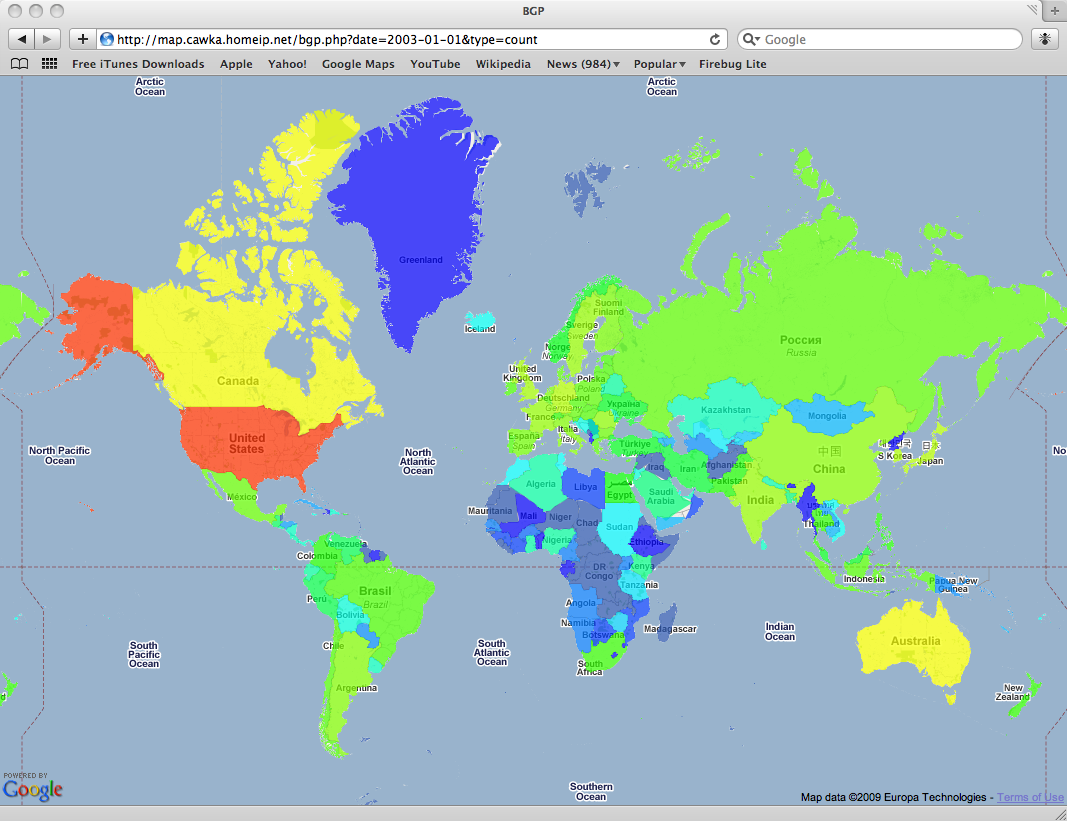
\includegraphics[trim=0 17px 0px 76px,clip=true,width=\columnwidth]{00_maps/bgp_count_2003}%
		\hspace{-0.98\columnwidth}%
		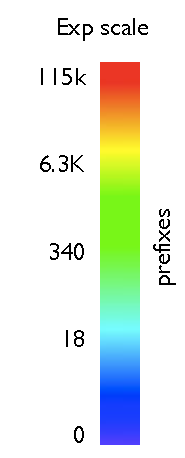
\includegraphics[width=1cm]{scale_bgp_count}\hspace{-1cm}%
		\hspace{0.98\columnwidth}
	\caption{Geographical distribution of number of announced prefixes on \textbf{January 1, 2003}}
	\label{fig:bgp prefixes 2003}
% \end{figure}
\end{minipage}%
%
\quad
%
\begin{minipage}[b]{0.48\textwidth}
% \begin{figure}[p]
	\centering
		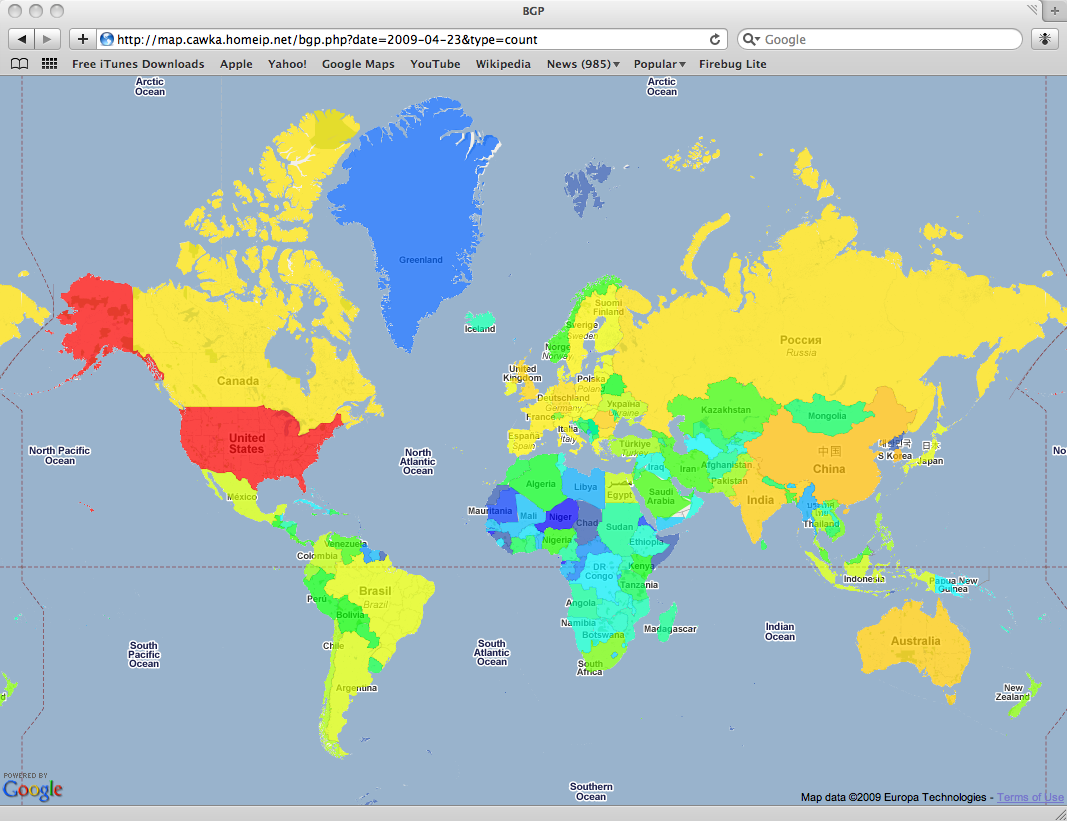
\includegraphics[trim=0 17px 0px 76px,clip=true,width=\columnwidth]{00_maps/bgp_count_2009_2}%
		\hspace{-0.98\columnwidth}%
		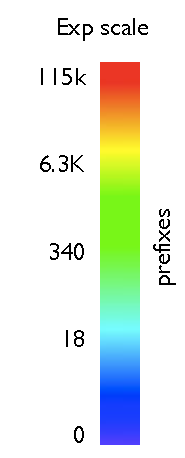
\includegraphics[width=1cm]{scale_bgp_count}\hspace{-1cm}%
		\hspace{0.98\columnwidth}
	\caption{Geographical distribution of number of announced prefixes on \textbf{April 23, 2009}}
	\label{fig:bgp prefixes 2009}
% \end{figure}
\end{minipage}

\vspace{0.5cm}

%%%%%%%%%%%%%%%%%%%%%%%%%%%%%%%%%%%%%%%%%%%%%%%%%%%%%%%%%%%%%%%%%%
%% BGP sizes
%%%%%%%%%%%%%%%%%%%%%%%%%%%%%%%%%%%%%%%%%%%%%%%%%%%%%%%%%%%%%%%%%%
\begin{minipage}[b]{0.48\textwidth}
% \begin{figure}[p]
	\centering
		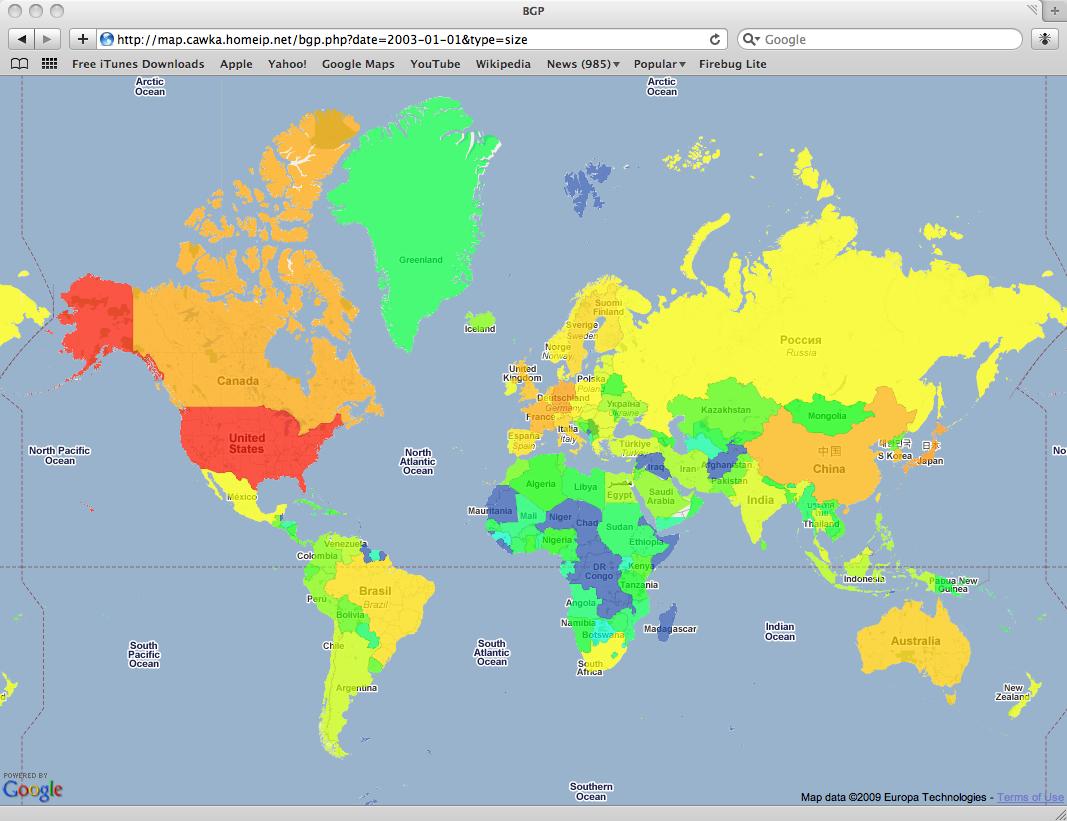
\includegraphics[trim=0 17px 0px 76px,clip=true,width=\columnwidth]{00_maps/bgp_size_2003}%
		\hspace{-0.98\columnwidth}%
		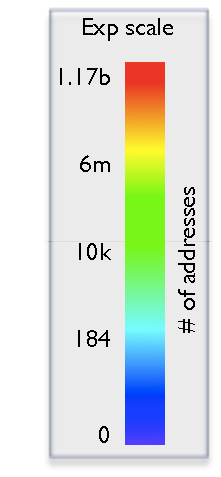
\includegraphics[width=1cm]{scale_bgp_size}\hspace{-1cm}%
		\hspace{0.98\columnwidth}
	\caption{Geographical distribution of announced IP space on \textbf{January 1, 2003}}
	\label{fig:bgp ip space 2003}
% \end{figure}
\end{minipage}%
%
\quad
%
\begin{minipage}[b]{0.48\textwidth}
% \begin{figure}[p]
	\centering
		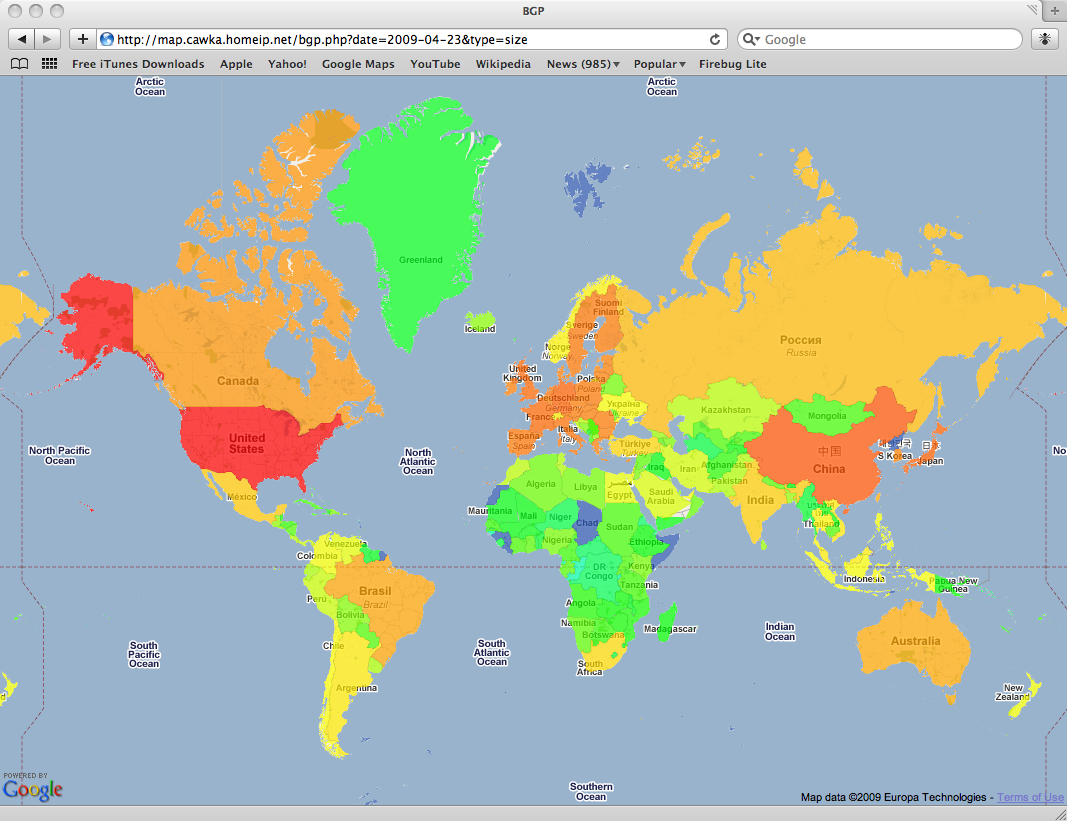
\includegraphics[trim=0 17px 0px 76px,clip=true,width=\columnwidth]{00_maps/bgp_size_2009_2}%
		\hspace{-0.98\columnwidth}%
		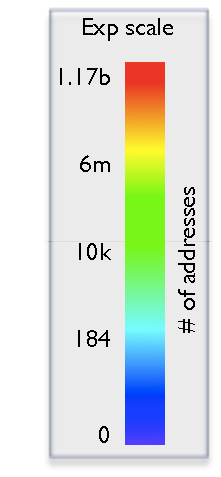
\includegraphics[width=1cm]{scale_bgp_size}\hspace{-1cm}%
		\hspace{0.98\columnwidth}
	\caption{Geographical distribution of announced IP space on \textbf{April 23, 2009}}
	\label{fig:bgp ip space 2009}
% \end{figure}
\end{minipage}

\vspace{0.5cm}

%%%%%%%%%%%%%%%%%%%%%%%%%%%%%%%%%%%%%%%%%%%%%%%%%%%%%%%%%%%%%%%%%%
%% Asia region
%%%%%%%%%%%%%%%%%%%%%%%%%%%%%%%%%%%%%%%%%%%%%%%%%%%%%%%%%%%%%%%%%%
\begin{minipage}[b]{0.48\textwidth}
% \begin{figure}[p]
	\centering
		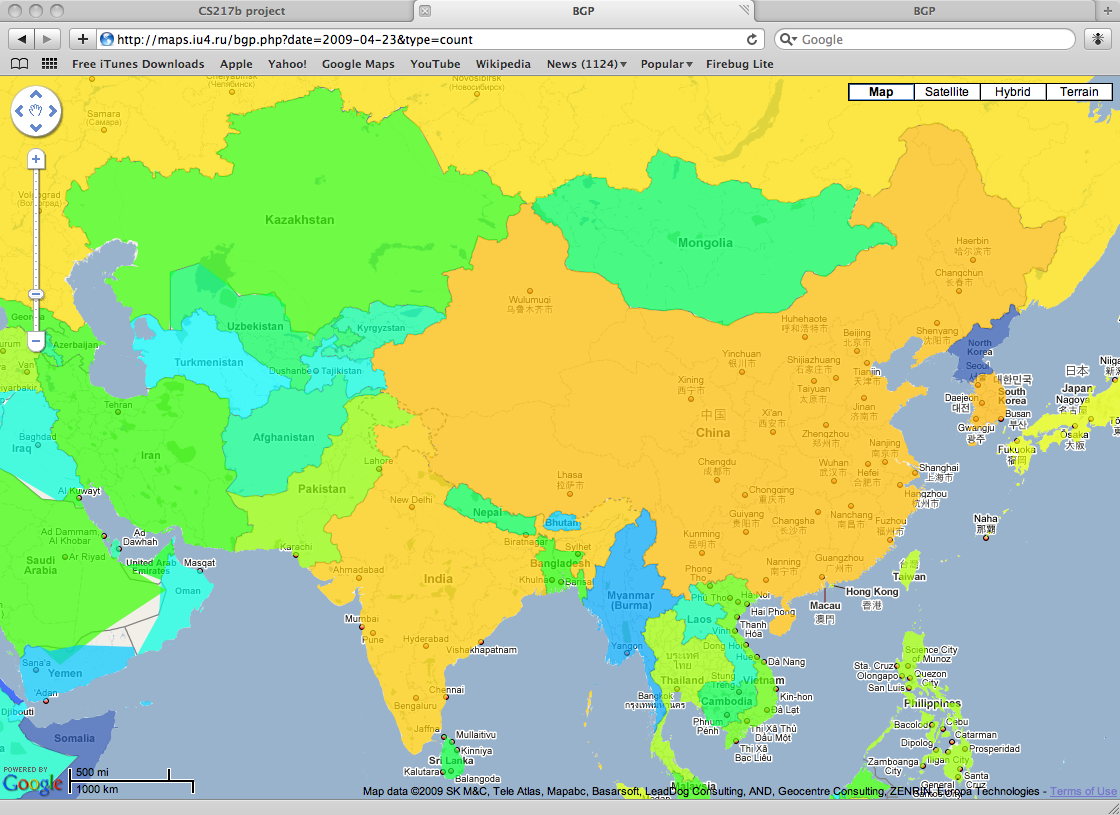
\includegraphics[trim=0 17px 0px 76px,clip=true,width=\columnwidth]{00_maps/asia_2009_prefixes}%
		\hspace{-0.98\columnwidth}%
		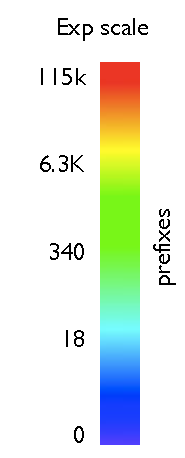
\includegraphics[width=1cm]{scale_bgp_count}\hspace{-1cm}%
		\hspace{0.98\columnwidth}
	\caption{Geographical distribution of number of announced prefixes in Asian region on \textbf{April 23, 2009}}
	\label{fig:bgp prefixes asia 2009}
% \end{figure}
\end{minipage}%
%
\quad
%
\begin{minipage}[b]{0.48\textwidth}
% \begin{figure}[p]
	\centering
		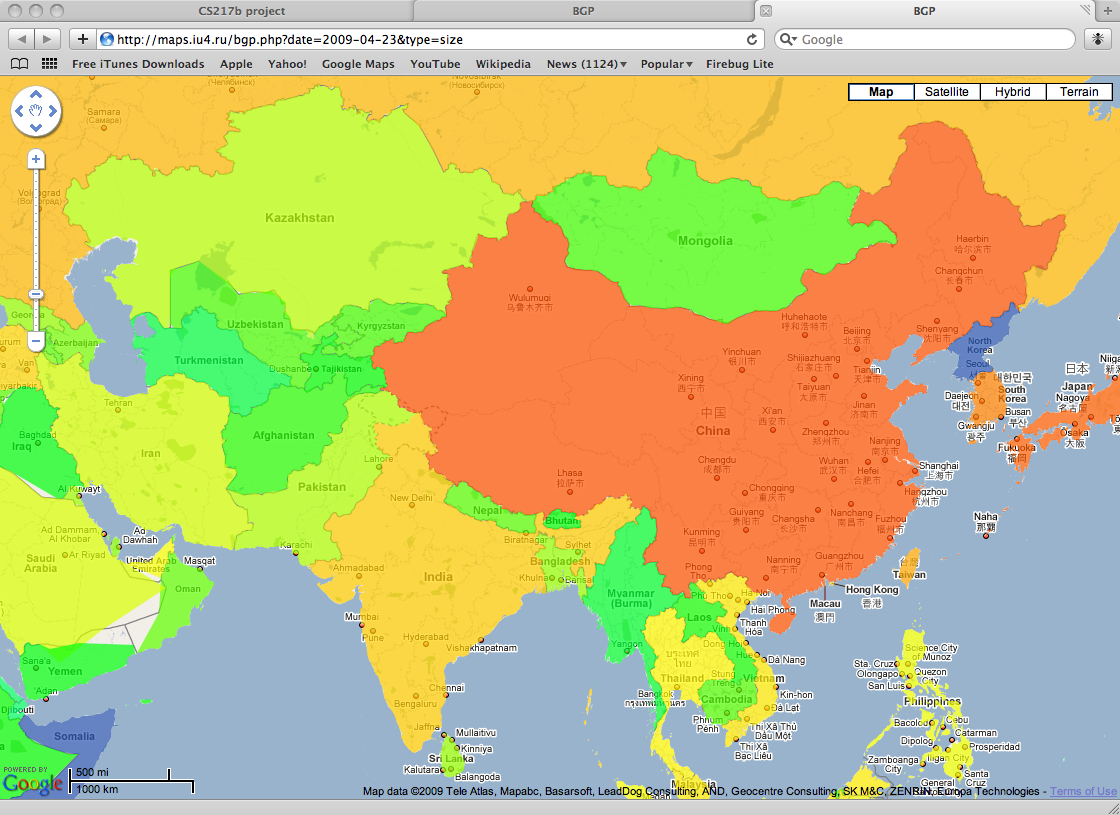
\includegraphics[trim=0 17px 0px 76px,clip=true,width=\columnwidth]{00_maps/asia_2009_space}%
		\hspace{-0.98\columnwidth}%
		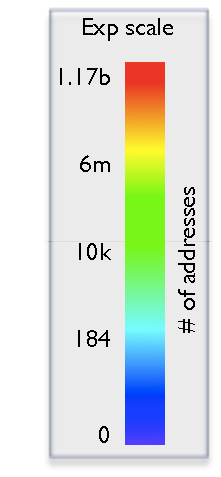
\includegraphics[width=1cm]{scale_bgp_size}\hspace{-1cm}%
		\hspace{0.98\columnwidth}
	\caption{Geographical distribution of announced IP space in Asian region on \textbf{April 23, 2009}}
	\label{fig:bgp ip space asia 2009}
% \end{figure}
\end{minipage}

\end{figure*}

% \clearpage

